\section{Graphs, Cliques, Stable Sets and Entropy}
\label{tree:poset:graph}

We now focus on how to define the information a poset contains. Obviously, in
our decision tree model, a totally ordered set contains maximum information
while a totally unordered set contains no information at all. We have to
understand it this way: if we want to sort a poset, sorting it means acquiring
information on the relation $\le$. If our poset is totally ordered, then we
have all the information needed to describe the relation $\le$ completely. If
the poset contains no information at all, then it means any first $x \ask{\le}
y$ question we might ask gives us exactly $1$ bit of information. In other
words, we cannot deduce any $x \le y$ relation from this poset. Hence, it is
totally unordered.

\subsection*{(In)Comparability Graphs}

To help understand the structure of a poset we introduce the comparability
graph ${G}(\P)$ and the incomparability graph $\widetilde{G}(\P)$.

Formally,

\begin{quotation}
The comparability graph ${G}(\P)$ of a poset $\P$ is an undirected graph whose
vertices are the poset elements, and in which two vertices are adjacent if and
only if the elements are comparable.
\end{quotation}

\begin{quotation}
The incomparability graph $\widetilde{G}(\P)$ of a poset $\P$ is an undirected
graph whose vertices are the poset elements, and in which two vertices are
adjacent if and only if the elements are incomparable.
\end{quotation}



Those graphs explicitly represent all relations (or pairs of incomparable
elements) which may be inferred from the Hasse diagram of $\P$. For example,
the comparability graph of a totally ordered set is the complete graph. See
\ref{fig:comp-graph} for a visual example.

\nb{Note that, by abuse of notation, we write $G$ instead of ${G}(\P)$.}


\begin{figure}
\centering
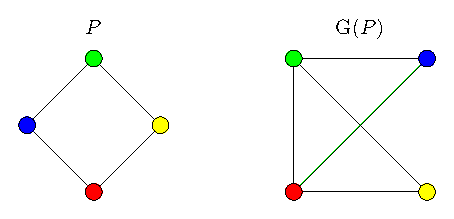
\includegraphics[height=0.2\textheight]{fig/comp-graph}
\caption{\label{fig:comp-graph} A Hasse diagram and its comparability graph.}
\end{figure}




\subsection*{Cliques and Stable Sets}


Now that we have new tools to represent a poset, we are interested in analyzing
remarkable structures like we did before for Hasse diagrams. Indeed, we define
hereunder the counterparts of chains and antichains in posets for
(in)comparability graphs.

\begin{quotation}
A clique $\C$ of graph $G$ is a subset of pairwise adjacent vertices in $G$,
i.e. the subgraph induced by $\C$ is complete.
\end{quotation}

A clique in a comparability graph ${G}$ is a subset of comparable elements in
$\P$, i.e. a chain in $\P$.

A clique in an incomparability graph $\widetilde{G}$ is a subset of
incomparable  elements in $\P$, i.e. an antichain in $\P$.

\begin{quotation}
A set $\S$ is stable (or independent) if the vertices in $\S$ are pairwise
nonadjacent, i.e. the subgraph induced by $\S$ has $\card{\S}$ connected components.
\end{quotation}

A stable set in a comparability graph ${G}$ is a subset of incomparable
elements in $\P$, i.e. an antichain in $\P$.

A stable set in an incomparability graph $\widetilde{G}$ is a subset of
comparable elements in $\P$, i.e. a chain in $\P$.


\nb{A stable set in ${G}$ is a clique in $\widetilde{G}$ and vice versa.}



\subsection*{$\operatorname{STAB}(G)$}
\label{tree:poset:graph:stab}

In what follows we show that from the internal structure of a graph $G$
expressed using its stable sets we can deduce a discrete distribution
look-alike object. With the help of this object we are able to compute the
entropy of graph $G$.

Let us suppose we want to describe our graph $G$ by a \emph{composition of the
stable sets it contains}. This leads us to define \emph{the set of convex
combinations of stable sets} of $G$. We call it $\operatorname{STAB}(G)$.
$\operatorname{STAB}(G)$ is a set containing all convex combinations (positive,
coefficients summing up to $1$) of characteristic vectors $\chi^{\S}$, where $\S$
is a stable set. $\chi^{\S}$ is a point in $\R^n$ where

$$ \chi^{\S}_v =\begin{cases}
      1, & \text{if}\ v \in \S\\
      0, & \text{otherwise}.
    \end{cases}$$


In other words $\chi^{\S}$ is a binary inclusion/exclusion representation of the
stable set $\S$.
\begin{equation}
\operatorname{STAB}(G) \bydef \operatorname{conv}\enum{\chi^{\S} \in \R^V \st
\S\text{ stable set in }G}
\label{eq:stab}
\end{equation}

Formally, \ref{eq:stab} is the definition of the \emph{stable set polytope} of
an arbitrary graph $G$ with vertex set $V = \enum{v_1, \ldots, v_n }$
and order $n$ ($\R^V = \R^n, n = \card{V}$) i.e. the convex hull (an $n$-dimensional
polytope) of stable set characteristic vectors $\chi^{\S} \in \R^n$.



\subsection*{Entropy for Comparability Graphs}

The entropy of a graph can be defined in several ways (see
\citet*{mowshowitz2012entropy} and \citet*{simonyi1995graph}). One idea would
be to look at a given feature of a graph (e.g. the number of edges) and then
define the entropy of this graph to be some function of this feature.

Here we define the entropy of a comparability graph $G$ as a function of the
stable sets $G$ possesses. In order to do so, we look at every vector in
$\operatorname{STAB}(G)$ and we keep the vector that gives the lowest entropy
value for a given entropy function. This vector is the discrete distribution
look-alike object we talked about in \ref{tree:poset:graph:stab} and the
entropy value is called the entropy of graph $G$, denoted ${H}(G)$.

Formally, we define the entropy of comparability graph $G$ as

\begin{equation}
{H}(G) \bydef \min_{x \in \operatorname{STAB}(G)}~ -\frac{1}{n} \sum_{v \in
V} \log x_v.
\label{eq:entropy:graph}
\end{equation}

Note that any $x^*$ which minimizes \ref{eq:entropy:graph} also minimizes the
sum on $\log \frac{1}{x_v}$.



\subsection*{Entropy for Posets}


As we defined ${H}(G)$ in \ref{eq:entropy:graph}, we write ${H}(\P)$ to mean
${H}(G(\P))$.

\begin{equation}
{H}(\P) \bydef {H}({G}(\P)).
\label{eq:entropy:poset}
\end{equation}
